%---------| background outline |---------%
%---------| 1. Define what model-based controls is
\subsection{Model-based Controls in Soft Robotics}
Much of controls theory as a field has progressed in parallel to the advances in our understanding of dynamic modeling. In fact, much of the advancements in controls theory were driven by the need to supplement the gaps in our dynamic models. Starting from the frequency domain and linear controllers, to nonlinear controllers, and most recently machine learning. 

The implementation of control strategies for standard rigid robots has followed this line of progression. Algorithms built around the dynamical model of the robot itself came first, then only recently did strategies employing machine learning began to be implemented--mostly to handle unpredictable scenarios beyond the models' assumptions. Control strategies of the former kind are known as \textit{model}-based controls, where controllers are designed based on models that mathematically represent the robot's dynamics \cite{rakhmatillaev_integrative_2025}. It should be apparent that this has been the case since the dynamics of a rigid-bodied robot can more readily be modelled. 

On the other hand, the development of control strategies for \textit{soft} robots have followed the opposite direction: much of the early works in soft robotics controls employed machine learning strategies due to the high level of complexity and dimensionality required in the dynamical models. Thus, \textit{learning}-based controls were the model for soft robot control strategies through the formative years of the field. Only in recent years did this precedent began to be re-assessed, particularly with the advent of \textit{finite}-dimensional modelling (FDM) techniques compatible with the continuum dynamics of soft robots \cite{della_santina_model-based_2023}.
%----------------------------------------%     
%---------| 2. Model-based vs, learning-based; 
\subsection{Model- vs. Learning-based Controls}
Model- and learning-based controls differ in the fundamental methodology that underpin \textit{how} each approach steers their dynamic systems. Consider some steady-state open-loop dynamic system expressed in state space as $\mathbf{\dot{x}}=\mathbf{f}(\mathbf{x})$, the application of a model- and learning-based controller--respectively--to the system may be represented according to \autoref{modelvslearn}.

\def\sysDyTerms{
    \underline{\dot{q}}=\mathbf{f}(\underline{q},\underline{u})
}

\begin{table}[!ht]
    \centering
    \begin{tabularx}{0.9\textwidth}{|*{2}{>{\centering\arraybackslash}X|}}
        \hline
        Model-based & Learning-based \\
        \hline
        \raggedright Given \par 
        \centering\arraybackslash $\begin{aligned}
            \sysDyTerms & \xrightarrow[\text{for}]{\text{solve}} \underline{u}(\underline{q},\underline{\bar{q}},...)\\
            \mathbf{f}(\underline{q},\underline{u}) & \rightarrow \mathbf{f}(\underline{q},\underline{u}(\underline{q},\underline{\bar{q}}))
        \end{aligned}$ \par
        \raggedright Such that \par 
        \centering\arraybackslash $\underline{\dot{q}} \approx \underline{\bar{\dot{q}}}$ \par & 
        \raggedright Given some dataset \par 
        \centering\arraybackslash 
            $X = \{(\underline{q_0},\underline{u_0}),\dots,(\underline{q_i},\underline{u_i})\}$ \par
        $\begin{aligned}
            X & \xrightarrow[\text{from}]{\text{extract}} \underline{u}^{\text{learned}}
        \end{aligned}$ \par
        \raggedright Such that \par
        \centering\arraybackslash
            $\underline{\dot{q}} \approx \underline{\bar{\dot{q}}}$ \\
        \hline
    \end{tabularx}
    \caption{High-level generalization of model- vs. learning-based controllers, where $\underline{\bar{\dot{q}}}$, $\underline{\bar{q}}$ describes the desired/reference configuration.}
    \label{modelvslearn}
\end{table}

% \raggedright\arraybackslash Where $\underline{\bar{\dot{q}}}$, $\underline{\bar{q}}$ describes the desired/reference configuration

The distinction between model- and learning-based control approaches may be described using the functional framework presented above. In both approaches, some input $\mathbf{u}$ is now introduced to the previously steady-state system. The system becomes \textit{closed}-loop when a controller that uses the system output to determine the control input is implemented (see \autoref{openvsclosed}). %<-- need diagram to help explain!
In this scenario, $f(\mathbf{x,e,t,...})$ can be considered the controller. It functionally relates the system output/current state--and typically error $\mathbf{e}$ and time as well--to the control input. 

\begin{figure}[h!]
    \centering
    \begin{tikzpicture}
        \bXInput[$\mathbf{r}$]{a}
        \bXComp*{b}{a}{}{-}{+}{}
        \bXLink{a}{b}
        \bXBlocL[3]{c}{
            $\mathbf{u}=f(...)$        
        }{b}
        \bXLinkName[0.7]{b-c}{$\mathbf{e}$}
        \bXLinkName[2.5]{c}{Controller}
        \bXBlocL[3]{d}{
            $\mathbf{\dot{x}=Ax + Bu}$
        }{c}
        \bXLinkName[0.7]{c-d}{$\mathbf{u}$}
        \bXLinkName[2.5]{d}{System}
        \bXOutput[4]{e}{d}
        \bXLink{d}{e}
        \bXLinkName[0.7]{d-e}{$\mathbf{x}$}
        \bXBranchy{d-e}{f}
        \bXBlocr[8]{g}{Feedback}{f}
        \bXLinkyx{d-e}{g}
        \bXLinkxy{g}{b}
    \end{tikzpicture}
    \caption{A generic closed-loop system, the control input is a function of desired state $\mathbf{r}$ and output $\mathbf{x}$.}
    \label{openvsclosed}
\end{figure}


For model-based controls, designing the controller based on the dynamics of the systems means tuning $\mathbf{u}$ to the $\mathbf{A}$ and $\mathbf{B}$ matrices. A conveniently acceptable way of interpreting $\mathbf{\bar{f}}$ is to regard $\mathbf{A}$ as the system's steady-state behavior, and $\mathbf{B}$ as the system's response to control inputs. The two matrices \textit{must} sufficiently describe the system dynamics before $\mathbf{u}$ can be designed to steer the system towards the desired configuration. Formulating $\mathbf{A}$, $\mathbf{B}$, and $\mathbf{u}$ while respecting their inter-dependency thus becomes inherent to the model-based approach.
  
Formulating models that allow the input to be solved in a mathematically managable way, while simultaneously remaining faithfully representative of the \textit{actual} system behavior becomes one of model-based controls' biggest challenges. Learning-based controls circumvent this by using data-driven techniques and learning algorithms to arrive at $\mathbf{u}$. In some cases, $\mathbf{\bar{f}}$ may even be left unknown and the full system is wholly formulated by the learning medium ($\mathbf{g(x,u)}$ in \autoref{modelvslearn}).

\begin{comment} 
    Learning-based controllers have been known to achieve higher levels of performance with respect to more complex actions, typically at the cost of computational efficiency and/or formal guarantees of safety for the robot's behavior \cite{brunke_safe_2022}. Since the formulation of $\mathbf{g(x,u)}$ and $u_{\text{learned}}$ is handled by the learning medium, we are left without the ability to extract detailed functional information regarding either of them. 
\end{comment}
\begin{table}[h!]
    \centering
    \begin{tabularx}{\textwidth}{
        >{\hsize=0.2\hsize\centering\arraybackslash}X|
        >{\hsize=0.4\hsize\centering\arraybackslash}X|
        >{\hsize=0.4\hsize\centering\arraybackslash}X
        }
        Analysis        & Model-Based & Learning-Based\\ \hline\hline
        \raggedleft Advantages      & 
        Meaningful information regarding the dynamics and inputs of the system are preserved &
        Known to achieve higher maneuvering performance and better robustness\newline
        \cite{rakhmatillaev_integrative_2025}\\ \hline
        \raggedleft Disadvantages   &
        Less robust and adaptable at handling system configurations in fringe scenarios\newline
        \cite{rakhmatillaev_integrative_2025}, \cite{brunke_safe_2022} &
        More complex and typically lacks formal guarantees of safety\newline
        \cite{brunke_safe_2022}\\
    \end{tabularx}
    \caption{An assessment of Model- and Learning-Based controls.}
    \label{comparison}
\end{table}

A general assessment of the benefits and drawbacks between the two approaches is presented in \autoref{comparison}. While both approaches bring different things to the table--and extensive research continue to be conducted on both, the author has decided to explore the model-based approach for this proposed thesis.
%----------------------------------------%  
%---------| 3. Brief overview/lit. review of contemporary models
\subsection{Some "Control-Oriented" Models}
It was mentioned earlier that in the formulation of the dynamical model to develop a controller around, towing the balance between mathematical simplicity and physical accuracy is one of the major challenges in model-based controls. While this continues to be true, continuum dynamics-compatible FDM techniques has also indeed broken considerable ground with regards to this issue. In their exact formulation, the dynamics of a soft robot is effectively an infinite-dimensional system. Such a system cannot be described without the use of partial differential equations (PDEs). However, by applying the appropriate assumptions, approximations, and/or discretization to the dynamical model of the soft robot, the system's description may be reliably "minimized" into a \textit{finite}-dimensional system that can be described with ordinary differential equations (ODEs) instead.

One of the most widely-implemented family of FDM techniques is the Piecewise Constant Strain (PCS) approximations (see \autoref{rodandpcs}). It is a family of discretization methods applied to a type of approximation for soft robot dynamics known as "rod models". It is extremely common for soft robots to be "thin" and/or "elongated": to have one physical dimension dominate the other two. In that regard, such soft robots may be approximated as a rod with the continuum mechanics of one too--hence rod models. At the heart of this methodology is the assumption that volumetric deformations may be neglected, and modeling the dynamics around the dominant central axis is sufficient \cite{della_santina_model-based_2023}.

\begin{figure}[h!]
    \centering
    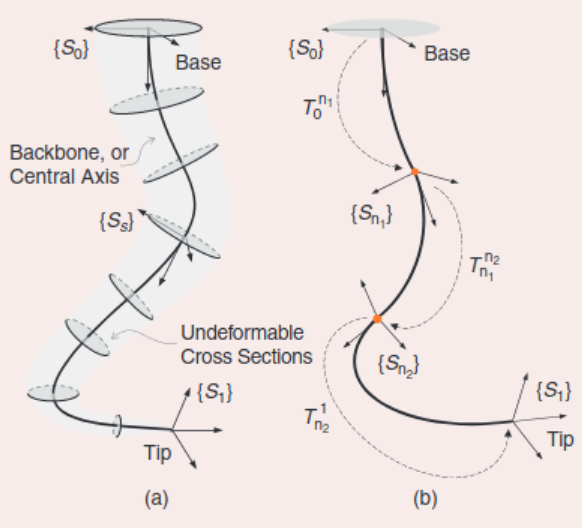
\includegraphics[width=0.4\textwidth]{graphics/rodandpcs.png}
    \caption{a) "Elongated" soft robots as described in rod models. b) PCS discretization applied to the rod model. Image taken from Della Santina et al. \cite{della_santina_model-based_2023}.}
    \label{rodandpcs}
\end{figure}

Among the many implementations of PCS, the planar Piecewise Constant Curvature (PCC) model has been extensively used in soft robotics throughout the last decade. Its approximation of the robot as pieces of constant-curvature arcs linked together in series with mutually tangent connection points makes the kinematics and Jacobian formulation for the model \textit{closed}-form \cite{websteriii_design_2010}. A dynamic feedback controller using this model was developed in \cite{della_santina_model-based_2020}, with an implementation of a trajectory generator for the controller formulated in \cite{dickson_real-time_2025}. 

There are many viable models out there that can be used as the basis for the controller that this proposed thesis seeks to develop, a selection of them that seems promising with respect to the scope of this proposed thesis will be outlined in this proposal.